\section{First Exercise}
Firstly the NAND-gate looks like
\begin{figure}[H]
    \singlespacing
    \begin{subfigure}[]{0.45\textwidth}
        \flushright
        \includegraphics{nand.pdf}
    \end{subfigure}
    \hfill
   \begin{subtable}[]{0.45\textwidth}
        \flushleft
        \begin{tabular}{ccc}
            \toprule
           $A$ & $B$ & $C$\\
            \midrule
            0 & 0 & 1\\
            0 & 1 & 1\\
            1 & 0 & 1\\
            1 & 1 & 0\\
            \bottomrule
            
        \end{tabular}
   \end{subtable}
   \caption{NAND-gate and the corresponding truth table.}
\end{figure}
Now we can easily make the AND-gate
\begin{figure}[H]
    \singlespacing
    \begin{subfigure}[]{0.45\textwidth}
        \flushright
        \includegraphics{and.pdf}
    \end{subfigure}
    \hfill
   \begin{subtable}[]{0.45\textwidth}
        \flushleft
        \begin{tabular}{ccc}
            \toprule
            $A$ & $B$ & $C$\\
            \midrule
            0 & 0 & 0\\
            0 & 1 & 0\\
            1 & 0 & 0\\
            1 & 1 & 1\\
            \bottomrule
            
        \end{tabular}
   \end{subtable}
   \caption{AND-gate and the corresponding truth table.}
\end{figure}
As well as the NOT-gate
\begin{figure}[H]
    \singlespacing
    \begin{subfigure}[]{0.45\textwidth}
        \flushright
        \includegraphics{not.pdf}
    \end{subfigure}
    \hfill
   \begin{subtable}[]{0.45\textwidth}
        \flushleft
        \begin{tabular}{cc}
            \toprule
            $A$ & $B$\\
            \midrule
            0 & 1\\
            1 & 0\\
            \bottomrule
        \end{tabular}
   \end{subtable}
   \caption{AND-gate and the corresponding truth table.}
\end{figure}
And finally the XOR-gate
\begin{figure}[H]
    \singlespacing
    \begin{subfigure}[]{0.45\textwidth}
        \flushright
        \includegraphics{xor.pdf}
    \end{subfigure}
    \hfill
   \begin{subtable}[]{0.45\textwidth}
        \flushleft
        \begin{tabular}{ccc}
            \toprule
            $A$ & $B$ & $C$\\
            \midrule
            0 & 0 & 0\\
            0 & 1 & 1\\
            1 & 0 & 1\\
            1 & 1 & 0\\
            \bottomrule
            
        \end{tabular}
   \end{subtable}
   \caption{XOR-gate and the corresponding truth table.}
\end{figure}